\subsection{Predicting vehicle state: the transition function}
\label{sec:vehicle_model_trans}

The aim of the prediction step is to obtain a \emph{prior predictive distribution} of the vehicle's state at time $\Vtime_k$ based on its previous state at time $\Vtime_{k-1}$, $p(\Vstate_k \cond{} \Vstate_{k-1})$. Using the model definition in \cref{eq:vehicle_model} along with the particle filter approximation of state in \cref{eq:vehicle_state_dirac}, we can write the prior prediction of the vehicle's state as
\begin{equation}
\label{eq:vehicle_pf_predict}
p(\Vstate_k \cond{} \Vstate_{k-1}) \approx
\sum_{i=1}^\Np
    \Pwt_{k-1}
    \DiracMeasure{\Vstate_k\vi}{\Vstate_k},
\end{equation}
where $\Vstate_k\vi = f(\Vstate\vi_{k-1}, \Vtdiff_k, \Vnoise)$ and $\Vtdiff_k = \Vtime_k - \Vtime_{k-1}$.

The transition function $\Vtrans$ is where we define the vehicle behaviours mentioned earlier. Kalman filter applications are limited to linear transformations of the state which can be expressed in a \emph{transition matrix}. However, \cref{eq:vehicle_pf_predict} shows that, in the case of the particle filter, the transition function is applied to each particle independently, allowing for a lot more flexibility in $\Vtrans$. We now describe the various model components of $\Vtrans$, implemented as an algorithm in the \pkg{transitr} package (see \cref{sec:particle-filter} for details). The core components are vehicle motion (speed and acceleration along a known path), stopping behaviour at known locations (bus stops and intersections), as well as the ability to handle several other scenarios to avoid degeneration.


\subsubsection{Component A: vehicle motion}
\label{sec:vehicle_model_behaviour}

The first behaviour to consider is the vehicle's motion along a known path: the \emph{speed} at which a vehicle is travelling will affect where it ends up. Since speed, $\Vspeed$, is the derivative of distance travelled over time, if $x = d(t)$, then $\Vspeed = d'(t)$, which is shown visually back in \cref{fig:vehicle_state}. It follows that we can predict a vehicle's future state, given its current state (distance travelled and speed) and system noise, $\Vnoise$, which is interpreted as \emph{the average change in speed per second}:
\begin{equation}
\label{eq:vehicle_model_newton}
\Vstate_{k|k-1} = f_{A1}\left(\Vstate_{k-1|k-1}, \Vtdiff_k, \Vnoise\right) =
\begin{bmatrix}
\Vdist_k \\ \Vspeed_k
\end{bmatrix} =
\begin{bmatrix}
\Vdist_{k-1} + \Vtdiff_k\Vspeed_k \\
\Vspeed_{k-1} + v_k
\end{bmatrix}
\end{equation}
where
\begin{equation}\label{eq:vehicle_model_newton_noise}
v_k \sim \TNormal{0}{\Vnoise}{-\Vspeed_{k-1}}{30 - \Vspeed_{k-1}}.
\end{equation}
The noise term is truncated to ensure the new speed is both positive and under 30~m/s, which is 108~km/h (the maximum road speed in Auckland is 100~km/h). The resulting transition function, $\Vtrans_{A1}$, is easily implemented by simulating, for each particle, a new speed before calculating the final state using \cref{eq:vehicle_model_newton}. A similar model was used by \citet{Cathey_2003,Dailey_2001}.


\Cref{fig:transition_demo} demonstrates transition model $\Vtrans_{A1}$ (left) using a sample of $N=10$~particles which, at time $t_{k-1}$, take one of three unique states (due to resampling in the previous iteration, \cref{sec:pf}). The points have been coloured by their initial state to demonstrate the effect of adding system noise \emph{before} transitioning to allow the particles to disperse. Not doing so would, in this instance, yield only three unique states in the final predictive distribution.

\begin{knitrout}\small
\definecolor{shadecolor}{rgb}{0.969, 0.969, 0.969}\color{fgcolor}\begin{figure}

{\centering 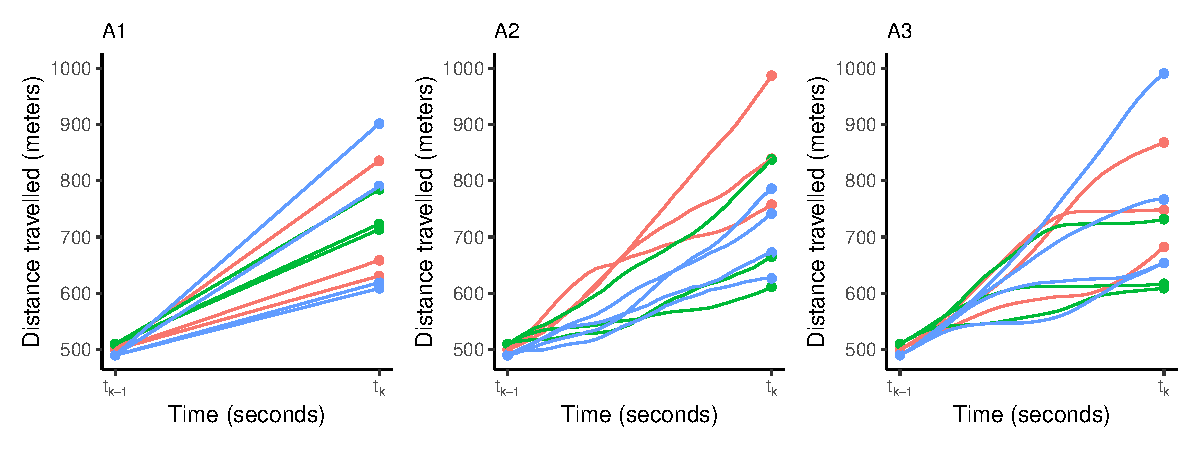
\includegraphics[width=\textwidth]{figure/transition_demo-1} 

}

\caption[Simulated particle trajectories using three transition functions]{Simulated particle trajectories using three transition functions, $f_{A1}$, $f_{A2}$, and $f_{A3}$ from left to right. Points have been coloured by their parent (after resampling) to demonstrate the affect of system noise.}\label{fig:transition_demo}
\end{figure}


\end{knitrout}

The main issue with this model is that it assumes constant speed between observations, which---given Auckland traffic---is unlikely to be the case. In \cref{fig:vehicle_state}, we showed speed varying over time, even between observations. To model this, we \emph{iteratively} update the vehicle's state\footnote{This is one advantage of the particle filter---we can easily perform iterative updates!} by reusing \cref{eq:vehicle_model_newton} $\Vtdiff_k$ times, setting $\Vtdiff_k=1$ in each iteration. The second graph in \cref{fig:transition_demo} shows the effect this has on the particles' trajectories.


Of course, if speed is the first derivative of the vehicle's trajectory function, then \emph{acceleration} is the second, $\Vaccel = d''(t)$. In this case, we add a third component to the vehicle's state and consider speed similarly to distance. The transition function
\begin{equation}
\label{eq:vehicle_model_newton_accel}
\Vstate_{k|k-1} = \Vtrans_{A3}\left(\Vstate_{k-1|k-1},\Vtdiff_k,\Vnoise\right)
\end{equation}
is iterative. It is initialised with $\bz_0 = \Vstate_{k-1|k-1}$ and repeated for $s = 1, \ldots, \Vtdiff_k$ to obtain $\Vstate_{k|k-1} = \bz_{\Vtdiff_k}$:
\begin{equation}
\label{eq:vehicle_model_newton_accel_iter}
\bz_s =
\begin{bmatrix}
z_s \\ z_s \\ z_s
\end{bmatrix} =
\begin{bmatrix}
z_{s-1} + \dot z_s \\
\dot z_{s-1} + \ddot z_s \\
\ddot z_{s-1} + v_s
\end{bmatrix}.
\end{equation}
System noise (interpreted as \emph{the average change in acceleration per second}) is applied to the acceleration term and truncated to ensure the speed remains positive and less than 30~m/s,
\begin{equation}
\label{eq:vehicle_model_accel_dist}
v_s \sim \TNormal{0}{\Vnoise}{-\dot z_{s-1} - \ddot z_{s-1}}{30 - \dot z_{s-1} - \ddot z_{s-1}}.
\end{equation}
These trajectories are shown in the third graph of \cref{fig:transition_demo}. The main issue with $\Vtrans_{A3}$ is that it is difficult to parameterize and constrain the acceleration to ensure speed remains within the interval $(0,30)$ while preserving the function's ability to generate plausible trajectories.



\subsubsection{Component B: stopping at nodes}
\label{sec:vehicle_model_nodes}

In \cref{sec:route-segments}, we discussed using a road network consisting of nodes---either bus stops or intersections---and the roads connecting them. This \emph{segmentisation} allows each route to be expressed as a \emph{sequence of nodes} and connecting \emph{road segments}. Component A of the transition model deals with vehicle behaviour along the road segments; we now examine bus behaviour at nodes.

There are two types of nodes in our framework: \emph{bus stops} where passengers can board and disembark, and \emph{intersections} where buses (and other road users) wait depending on congestion levels and traffic lights. In each case, the bus's behaviour involves:
\begin{enumerate}
\item if the bus stops:
    \begin{enumerate}
    \item deceleration to zero,
    \item wait, and
    \item acceleration to traffic speed;
    \end{enumerate}
\item otherwise, continue as though there is no node.
\end{enumerate}
Only step 1b depends on the type of node.



\paragraph{Bus stops}

A bus's wait time at a bus stop is referred to as \emph{dwell time} and consists of three phases \citep{Hans_2015,Robinson_2013,Meng_2013,Wang_2016}:
\begin{enumerate}[i.]
\item doors open;
\item passengers board and alight; and
\item doors close, and vehicle waits for a gap in the traffic.\footnote{In New Zealand, buses do not get right-of-way, so it is common for them to be stuck for a while in a bus bay.}
\end{enumerate}
Phases i and iii can be combined with 1a and 1c from above (deceleration and acceleration, respectively) into a single parameter, $\mindwell$, which is assumed constant across all buses, stops, and routes.


Phase ii includes the time taken for passengers to get on and off the bus, which varies significantly between stops, routes, and time of day. There are many ways to model service time: an exponential \citep{Hans_2015}, regression models \citep{Shen_2013}, or a real-time Kalman filter \citep{Shalaby_2004}. Here, I present a truncated Normal distribution using the mean and variance of historical dwell times, truncated at zero. The service time at stop $m$ along a route ($m=1,...,M-1$; dwell time does not apply to the last stop) is denoted $\pserve_m$, modelled by its mean and variance, $\dwell_m$ and $\dwellvar_m$, respectively, as estimated from historical data:
\begin{equation}
\label{eq:stop_dwell_time}
\pserve_m \sim \TNormal{\dwell_m}{\dwellvar_m}{0}{\infty}.
\end{equation}

For each bus stop, we also have a \emph{stopping probability} $\Prstop_m\in(0,1)$. For the first and last stops, $m\in\{1,M\}$, this is unity; for the remainder, we have no data with which we can reliably estimate $\Prstop_m$, so, for now, we assume all stops have the same values specified by a global $\Prstop$ parameter (see \cref{sec:pf_params} for details on this). The outcome of whether a bus stops at a bus stop, $p_m$, is a Bernoulli trial,
\begin{equation}
\label{eq:stop_pstop}
\Istop_m \sim \Bern{\Prstop_m}.
\end{equation}
The total dwell time of a bus at stop $m$ can be expressed as
\begin{equation}
\label{eq:stop_total_dwell_time}
\pdwell_m = \Istop_m (\mindwell + \pserve_m),
\end{equation}
which, under the particle filtering framework, is straightforward to implement. \Cref{fig:eta_dwell_times} displays the dwell time distribution at a stop.


\begin{knitrout}\small
\definecolor{shadecolor}{rgb}{0.969, 0.969, 0.969}\color{fgcolor}\begin{figure}

{\centering 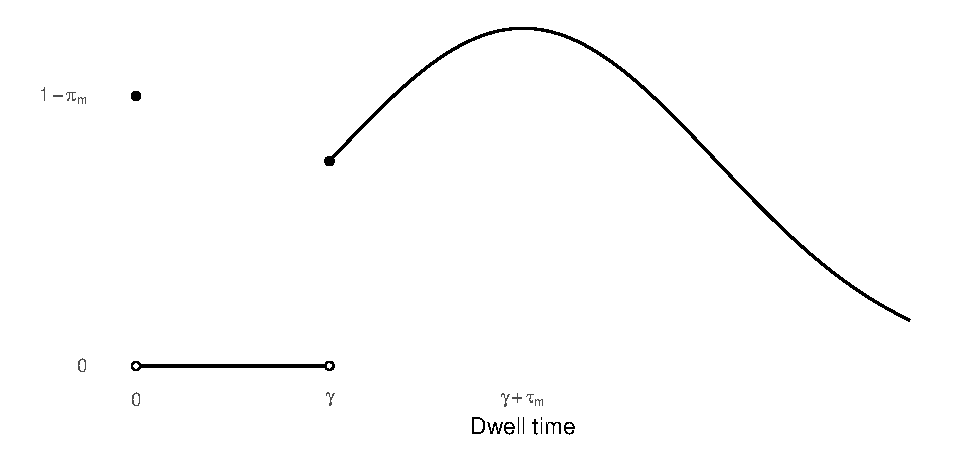
\includegraphics[width=.8\textwidth]{figure/eta_dwell_times-1} 

}

\caption[The \gls{pdf} of dwell time at a stop]{The \gls{pdf} of dwell time at bus stop $m$.}\label{fig:eta_dwell_times}
\end{figure}


\end{knitrout}


One other scenario for bus stops is a \emph{layover}, which is when a bus arrives early at a major stop\footnote{This is more common on longer routes in an attempt to keep them to schedule.} and waits until the scheduled departure time. In the \gls{gtfs} stop times table, layovers are denoted by an arrival time earlier than the corresponding departure time, as shown in \cref{tab:layover_times}. Again, under the particle filtering framework, this is simple enough to implement: if the particle arrives early, it waits until the scheduled departure time before leaving. However, it is not always the case that buses will wait for the layover, so we add a probability of adherence, similar to the stopping probability in \cref{eq:stop_pstop}. However, since this has greater implication for arrival time prediction, we defer the details for \cref{cha:prediction}.

\begin{knitrout}\small
\definecolor{shadecolor}{rgb}{0.969, 0.969, 0.969}\color{fgcolor}\begin{table}

\caption[Arrival times for a trip with a layover]{\label{tab:layover_times}Arrival times for a trip with a layover stop (marked with an asterix, $\star$). This is indicated in the \gls{gtfs} data by a departure time later than the arrival (in this case the difference is one second).}
\centering
\fontsize{8}{10}\selectfont
\begin{tabular}[t]{rll}
\toprule
Stop & Arrives & Departs\\
\midrule
1 & 19:30:00 & 19:30:00\\
2 & 19:30:36 & 19:30:36\\
3 & 19:31:33 & 19:31:33\\
4 & 19:32:04 & 19:32:04\\
5 & 19:32:59 & 19:33:00 *\\
6 & 19:33:42 & 19:33:42\\
7 & 19:34:14 & 19:34:14\\
\bottomrule
\end{tabular}
\end{table}


\end{knitrout}




\paragraph{Intersections}

Modelling intersections is much the same as bus stops, with a few differences:
\begin{enumerate}[i.]
\item the bus doors do not open, passengers do not get on or off, so there is no longer a $\gamma$ parameter;
\item the bus does not necessarily stop at the node location, since there may be a queue;
\item depending on the length of the queue and the type of intersection, the bus may require more than one ``light phase'' to pass through the intersection (for traffic lights), OR the bus may creep forward slowly (at uncontrolled (give-way) intersections and roundabouts).
\end{enumerate}
However, we had no reliable intersection location information available, so were unable to explore this component of the model thoroughly. Instead, I describe here a single behaviour but note that it could easily be modified in the future.

We model the wait time $w$ at intersection $\ell$ with an exponential distribution with rate $\intwait_\ell^{-1}$:
\begin{equation}
\label{eq:int_wait}
\pcwait_\ell \sim \Exp{\intwait_\ell^{-1}}.
\end{equation}
As at bus stops, the stopping outcome $\Iint_\ell$ is a Bernoulli trial with probability $\rho_\ell$,
\begin{equation}
\label{eq:int_stop_bern}
\Iint_\ell \sim \Bern{\rho_\ell},
\end{equation}
leading to an overall wait time of
\begin{equation}
\label{eq:int_total_wait}
\pwait_\ell = \Iint_\ell \pcwait_\ell.
\end{equation}
However, from point iii above, once the wait time is over, we conditionally allow the bus to move forward with the possibility of stopping again. In practice, this would be proportional to the distance of the vehicle from the intersection and other factors. As mentioned in \cref{sec:vp_data}, this is not as easy as it seems since observations may be linked to a waypoint at the intersection\footnote{Actually, in the middle of it.} instead of where the bus is, so we cannot determine the bus's distance from the intersection reliably.
